\documentclass[a4paper,11pt, twocolumn]{article}
\usepackage[margin=0.8in]{geometry}
\usepackage{xcolor}
\usepackage{graphicx} %package to manage images
\graphicspath{ {./images/} }

\title{A2-12 Further Semiconductor Components}
\author{Revision sheet}
\date{}

\usepackage{fancyhdr}
\pagestyle{fancy}
\fancyhead{} % clear all header fields
\renewcommand{\headrulewidth}{0pt} % no line in header area
\fancyfoot{} % clear all footer fields
\renewcommand{\footrulewidth}{0.4pt}
\fancyfoot[C]{\thepage} % page number in centre of the page
\fancyfoot[R]{\footnotesize Thomas Boxall \\ Images from WJEC E-Book} % right hand footer has author name on top line and images reference on bottom line
\fancyfoot[L]{\footnotesize A2-12 Further Semiconductor Components \\ Revision sheet} % left hand footer has title of document on top line and 'Revision Sheet' on bottom line


\begin{document}

\maketitle
\thispagestyle{fancy}

% CONTENTS OF THE REVISION SHEET HERE

\section{Conduction In Semiconductors}
All electronics device components are made of semiconductors.
\subsection{Materials}
There are three different types of materials in semiconductors.
A diagram called an \textit{Energy Band Diagram} can be used to show the energy level of electrons within types of materials. Electrons that have sufficient energy to escape from their `home' atom are found in the conduction band. Electrons with less energy cannot leave the valence band and be part of an electric current - they are found in the valence band and are known as valence electrons. 
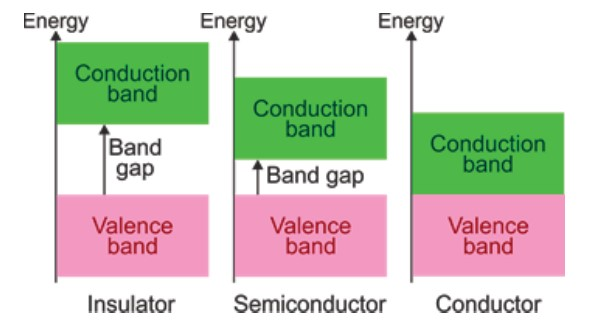
\includegraphics[width=\linewidth]{energyBandDiagram.jpg}
\subsection{Conductors}
In conductors, electrons don't need much energy to escape the atom therefore the material conducts at all temperatures.
\subsection{Insulators}
Electrons need a lot of energy to escape the atom therefore little-to-no  current flows.
\subsection{Semiconductors}
At room temperatures these are poor insulators and at warm temperatures they begin to conduct a little.
\subsection{Electrons And Holes}
At high temperatures, electrons can jump from the valence to conduction band. If we apply a voltage, then a current flows. This is known as Intrinsic Semiconductor Behaviour.
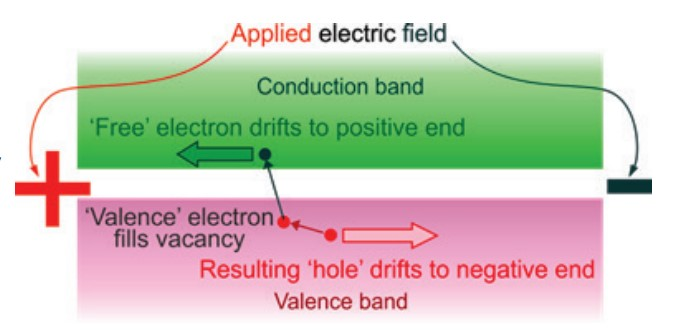
\includegraphics[width=\linewidth]{electronsAndHoles.jpg}
\subsection{Impurities}
The addition of impurities can change the electrical properties radically. This is very useful as new energy levels can be created.
\subsubsection{N-Type}
Add a new donor atom with one more electron than the semiconductor. This adds a free electron at a new energy level, close to the conduction band. 
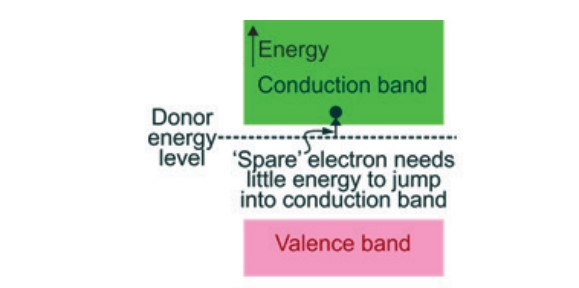
\includegraphics[width=\linewidth]{impureN.jpg}
\subsubsection{P-Type}
Add an acceptor atom with one less electron than the semiconductor. This adds a free hole at a new level close to the valence band.
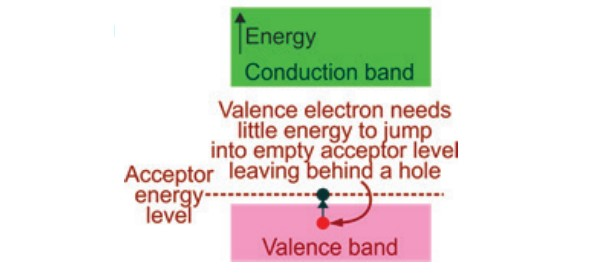
\includegraphics[width=\linewidth]{impureP.jpg}

\section{P-N Junction}
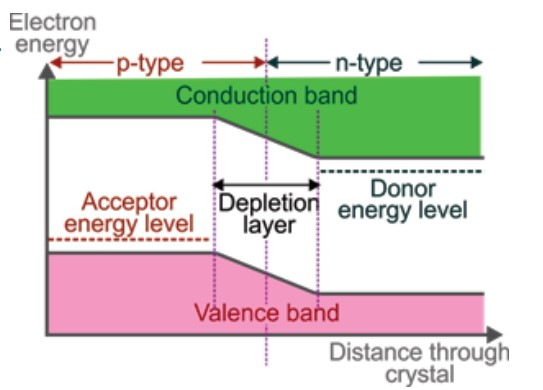
\includegraphics[width=\linewidth]{energyPN.jpg}
It is possible to combine two different impurities into one piece of semiconductor so that junctions can be formed, in this way a p-n junction can be formed. Electrons combine with holes therefore there are no charge carriers present at the point p and n meet, this is called the `depletion zone'. At the junction, a small battery is created, it has a voltage of 0.7V (called the potential barrier). This barrier is a barrier to electron flow as the negative ions repel electrons and positive ions repel holes.
\subsection{Forward Bias}
Apply a positive voltage to P, sucks free electrons toward depletion zone. Apply negative voltage to N, sucks holes towards depletion zone therefore current flows. Applied voltage has to be greater than 0.7V to get over potential barrier.
\subsection{Reverse Bias}
Positive voltage applied to N, pushes the holes back into P. Negative voltage applied to P, pushes electrons back into N.
\subsection{Conduction Diagram}
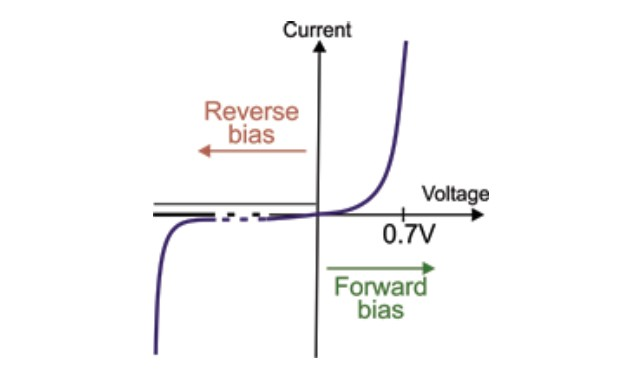
\includegraphics[width=\linewidth]{conductionDiagram.jpg}

\section{The MOSFET}
\textit{Metal Oxide Semiconductor Field Effect Transistor}. The diagram below shows the layout of the p and n regions.
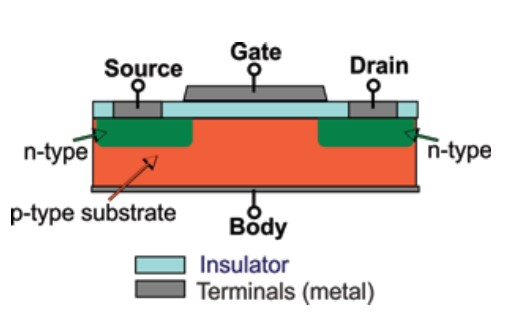
\includegraphics[width=\linewidth]{mosfet1.jpg}
This is an Enhancement Type N-Channel MOSFET. The p-region is very lightly doped therefore there aren't many free holes. With no gate voltage, no current flows. However when we apply a positive voltage to tha gate, electrons are attracted towards the gate and holes are pushed away, giving the following p and n region arrangement.
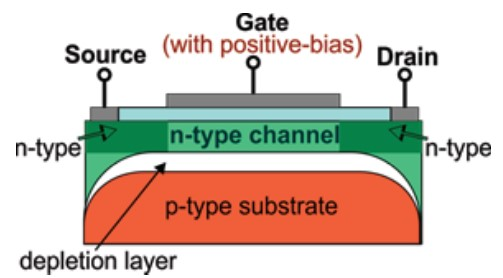
\includegraphics[width=\linewidth]{mosfet2.jpg}
This forms a conducting n-type channel between the source and drain (where the gate voltage greater than 3V).
\subsection{Properties Of MOSFETs}
They have a low on-resistance therefore they don't dissipate much power ($r_{DS_{ON}}$). They have an extremely high off-resistance. They have an infinitely high input resistance because the gate is insulated.

\end{document}